\hypertarget{part-2-image-1}{%
	\section{Part 2, Image 1}\label{part-1-design-2}}

\centering


\hypertarget{description}{%
	\subsubsection{Description}\label{description}}

\begin{description}
	\item[Image:]
	\item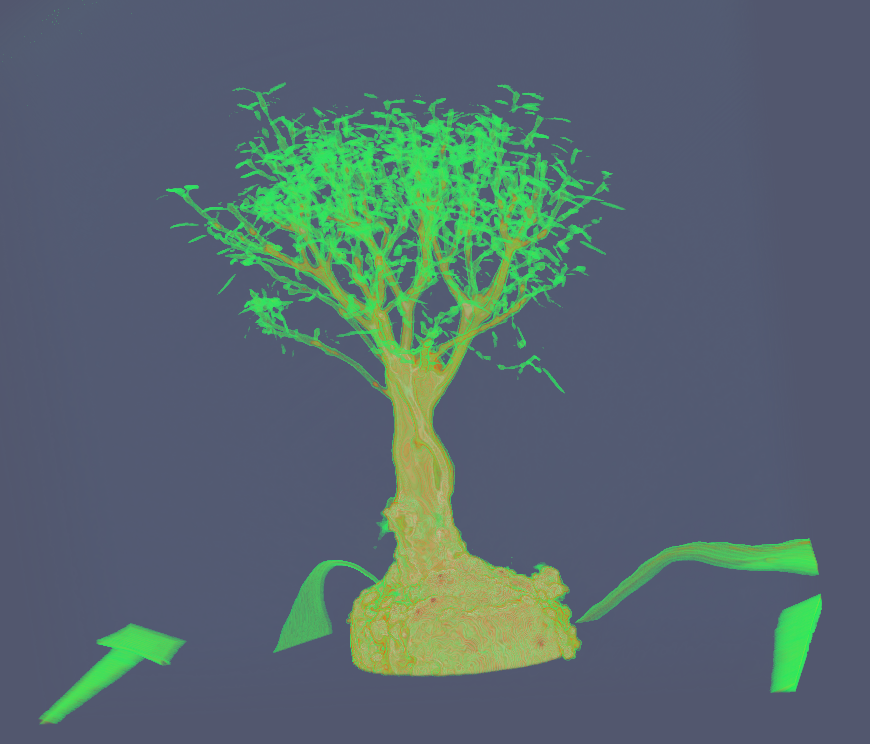
\includegraphics[width=12cm]{Tree1.png}
	
	\item[Tool:]
	\hfill \break 
		Paraview
	\item[Visual Mappings:]
	\begin{itemize}
		\tightlist
		\item[ ]
	\end{itemize}
	\begin{itemize}
		\tightlist
		\item
		\textbf{Mapping 1}:
		\hfill \break 
			Between data points 0.000 and 37.336, the opacity has been set to 0.000. At 38.336, the opacity has been assigned a value of 0.710, and this has been given a green colour, this is to get the leafs a green colour, and then goes back down to 0.000 opacity at data point 53.2243. While shooting up to data point 65.935 with an opacity of 0.208, then to data point 65.936 at opacity 0.664 with a reddish-brown colour assigned, this is to give the trunk of the tree a colour closely related to brown, this is more the outer layer of the tree trunk. Datapoint 89.766 assigned a green colour again with an opacity of 0.362, with an incline in opacity at data points 109.626 and 150.935, which have been assigned a deep drown colour having the values 0.505 and 0.731 in opacity, again to give the trunk an appearance of a brown colour. These are the more inner layers of the trunk. With then a slight decrease in opacity at data point 255.000 with an opacity of 0.000.
	\end{itemize}
	
	\begin{itemize}
		\tightlist
		\item
		\textbf{Mapping 2}:
		\hfill \break 
			LAB colour space used with a nan opacity of 1. A colour discretion has been used with a number of tables set to 256.
	\end{itemize}
	\item[Data Conversion:] 
	\hfill \break 
		Data scalar type unsigned char was used. Along with data extent: 0 - 511, 0 - 511, 0 - 181. Representation is set to volume with a volume rendering of OSPRay based and a blend mode of composite being used. File dimensionality is set to 3 and data byte order is set to BigEdndian.
	\item[Unique Observation:]
	\hfill \break
		Once the mapping has been altered a tree with leaves appears.
\end{description}